\documentclass{article}
\usepackage[utf8]{inputenc}
\setlength{\parskip}{5pt} % esp. entre parrafos
\setlength{\parindent}{0pt} % esp. al inicio de un parrafo
\usepackage{listings} % listings
\usepackage{color} %colores
\usepackage{amsmath} % mates
\usepackage[sort&compress,numbers]{natbib} % referencias
\usepackage{url} % que las URLs se vean lindos
\usepackage[top=15mm,left=20mm,right=20mm,bottom=25mm]{geometry} % margenes
\usepackage{hyperref} % ligas de URLs
\usepackage{graphicx} % poner figuras
\usepackage[spanish,es-tabla]{babel} % nombre tablas


\definecolor{mypink}{rgb}{0.976, 0.462, 0.847}
\definecolor{mygray}{rgb}{0.976, 0.980, 0.980}
\definecolor{myblue}{rgb}{0.258, 0.682, 1}
\definecolor{mypink2}{rgb}{0.525, 0.054, 0.4}
\lstset{ 
  backgroundcolor=\color{mygray},
  commentstyle=\color{myblue},
  keywordstyle=\color{mypink}, 
  numberstyle=\tiny\color{mypink}
  stringstyle=\color{mypink2}, 
  breaklines=true,
}


\title{Tarea 5}
\author{Eduardo Navarro}
\date{Septiembre 2021}

\begin{document}

\maketitle

\section{Introducción}
Siguiendo las indicaciones de la clase, se realizó una comparación entre un aproximado del valor del área de un integral, al cual le aplicamos pruebas estadísticas para ver el que tan mejor se aproxima nuestro resultado.

\section{Desarrollo}
Con las instrucciones de la tarea \cite{twitchsimu} se prosiguió a crear una instrucción para ver la similitud entre 2 cifras y que tan cercanas se encontraban a partir de sus decimales \cite{p}, agregándola al código que se nos proporcionó en \cite{montec} para ver la similitud entre la cifra generada y la calculada mostrada en \cite{montec}. Al programa se le añadieron \texttt{for} para los puntos y otro para las repeticiones dentro de éste. Se añadió un \texttt{for} adicional para la revisión de los decimales.


\begin{lstlisting} [language=R, caption= Código para la obtención de la relación entre los puntos y los decimales que coinciden.]
cuan <- c(100, 1000, 10000, 100000, 1000000, 10000000)
entero<- c(0.0488341111)
compar <- data.frame()
n = seq( 1, 10, 1)
j = c(1:50)

for (cuantos in cuan) {
  for (rep in j) {...
  
for (i in n) {
  e = trunc(entero*10^i)/10^i
  co = trunc(compa*10^i)/10^i
  if (co == e) {num = i
  } else {break;}
}

values<-c(cuantos, num)

compar=rbind(compar, values)
}
}
names(compar) <- c("puntos", "decimales")
\end{lstlisting}
\newpage
Con los datos obtenidos se obtuvo la tabla \ref{tabla1}, la cual nos sirvió para hacer nuestra gráfica \ref{grafica1} donde podemos observar un aumento en el número de decimales que coinciden en base al número de puntos.

\begin{table}[h!]
\centering
\caption{Muestra de datos obtenidos en comparación de decimales.}
\label{tabla1}
\begin{tabular}{|l|r|}
\hline
puntos & \multicolumn{1}{l|}{decimales} \\ \hline
100 & 1 \\ \hline
100 & 2 \\ \hline
100 & 1 \\ \hline
100 & 1 \\ \hline
100 & 1 \\ \hline
100 & 1 \\ \hline
100 & 2 \\ \hline
100 & 2 \\ \hline
100 & 1 \\ \hline
\end{tabular}
\end{table}

\begin{figure} [h!]% figura
\renewcommand{\figurename}{Gráfica}
    \centering
    \caption{Decimales que coinciden a partir de detreminado número de puntos.}
    \label{grafica1}
    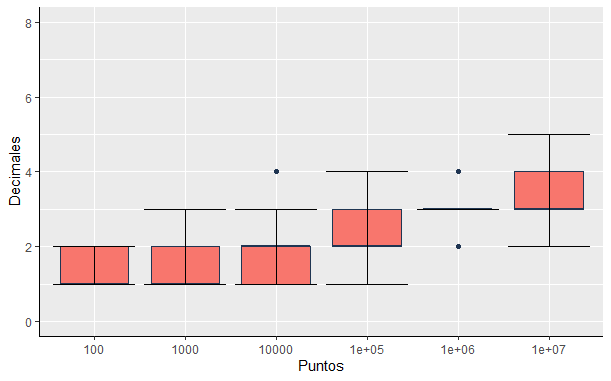
\includegraphics[width=120mm]{grafica1.png} % archivo
\end{figure}

\begin{lstlisting} [language=R, caption= Código para la obtención de la gráfica \ref{grafica1}.]
compar$puntos = as.factor(compar$puntos)

ggplot(compar, aes(x=puntos , y= decimales , fill= rep)) + # fill=name allow to automatically dedicate a color for each group
  geom_boxplot(fill = "#F8766D", colour = "#1F3552")+
  stat_boxplot(geom = "errorbar", width = 0.9)+
  theme(axis.line = element_line(colour = "black", size = 0.25))+
  coord_cartesian(ylim = c(0,8))+
  labs(x="Puntos", y= "Decimales")
\end{lstlisting}


A los datos de la tabla \ref{tabla1} se les hicieron las pruebas estadísticas de Shapiro–Wilk \cite{shapiro} y en base a los resultados obtenidos se realizó la prueba de Kruskal-Wallis \cite{Kruskall}.

\newpage

\begin{table}[h!]
\centering
\caption{Resultados de la prueba Shapiro–Wilk.}
\label{tabla2}
\begin{tabular}{|l|r|r|}
\hline
\multicolumn{1}{|c|}{puntos} & \multicolumn{1}{c|}{w} & \multicolumn{1}{c|}{p} \\ \hline
10\textasciicircum{}2 & 0.58795 & 1.295*10\textasciicircum{}-10 \\ \hline
10\textasciicircum{}3 & 0.6879 & 5.053*10\textasciicircum{}-9 \\ \hline
10\textasciicircum{}4 & 0.80305 & 1.031*10\textasciicircum{}-6 \\ \hline
10\textasciicircum{}5 & 0.83964 & 8.207*10\textasciicircum{}-6 \\ \hline
10\textasciicircum{}6 & 0.69368 & 6.384*10\textasciicircum{}-9 \\ \hline
10\textasciicircum{}7 & 0.76623 & 1.588*10\textasciicircum{}-7 \\ \hline
\end{tabular}
\end{table}

\begin{table}[h!]
\centering
\caption{Resultados de la prueba Kruskal-Wallis para todos los datos.}
\label{tabla3}
\begin{tabular}{|c|c|}
\hline
H(5) & p-value \\ \hline
180.72 & \multicolumn{1}{r|}{2.2*10\textasciicircum{}-16} \\ \hline
\end{tabular}
\end{table}

\begin{table}[h!]
\centering
\caption{Resultados de la prueba Kruskal-Wallis entre los últimos 2 datos.}
\label{tabla}
\begin{tabular}{|l|l|}
\hline
H(3) & p-value \\ \hline
3.9089 & 0.2715 \\ \hline
\end{tabular}
\end{table}

Se intentó el primer reto donde se tenía que verificar el valor de pi \cite{pi} obteniéndose la tabla \ref{tabla5} a la cual se le realizarón las pruebas estadísticas y finalmente se obtuvo la gráfica \ref{grafica2}. 

\begin{table}[h!]
\centering
\caption{Ejemplos de valores de pi obtenidos.}
\label{tabla5}
\begin{tabular}{|r|r|r|}
\hline
\multicolumn{1}{|l|}{valor pi} & \multicolumn{1}{l|}{puntos} & \multicolumn{1}{l|}{decimales} \\ \hline
3.124 & 10000 & 1 \\ \hline
3.154 & 10000 & 1 \\ \hline
3.1212 & 10000 & 1 \\ \hline
3.1556 & 10000 & 1 \\ \hline
3.1532 & 10000 & 1 \\ \hline
3.1188 & 10000 & 1 \\ \hline
3.146 & 10000 & 2 \\ \hline
3.1388 & 10000 & 1 \\ \hline
\end{tabular}
\end{table}

\newpage

\begin{figure} [h!]% figura
\renewcommand{\figurename}{Gráfica}
    \centering
    \caption{Decimales que coinciden en pi.}
    \label{grafica2}
    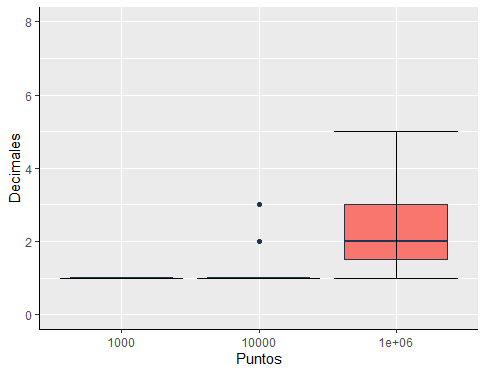
\includegraphics[width=120mm]{grafica2.png} % archivo
\end{figure}

\begin{table}[h!]
\centering
\caption{Resultados de la prueba Shapiro–Wilk para pi.}
\label{tabla6}
\begin{tabular}{|c|c|}
\hline
w & p \\ \hline
\multicolumn{1}{|r|}{0.60337} & \multicolumn{1}{r|}{8.386*10\textasciicircum{}-10} \\ \hline
\end{tabular}
\end{table}

\begin{table}[h!]
\centering
\caption{Resultados de la prueba Kruskal-Wallis para pi.}
\label{tabla7}
\begin{tabular}{|c|c|}
\hline
H(2) & p-value \\ \hline
\multicolumn{1}{|r|}{21.239} & \multicolumn{1}{r|}{2.44*10\textasciicircum{}-5} \\ \hline
\end{tabular}
\end{table}

\begin{lstlisting} [language=R, caption= Código para la obtención de pi.]

entero = 3.141592 
n = seq(1, 6, 1)
cuan = c(1000, 10000, 1000000)
compar = data.frame()
j = c(1:50)

for (cuantos in cuan) {
  for (rep in j){
    interior = 0
    for (r in 1:cuantos) {
      x = runif(1, -1, 1)
      y = runif(1, -1, 1)
      d = sqrt(x*x + y*y)
      if (d < 1) {
        interior = interior + 1
      }
    }
    
    tasa = interior / cuantos
    pi = 4 * tasa
    
    print(pi)
\end{lstlisting}

\section{Conclusiones}
Al obtenerse una p menor a 0.05 en la prueba de Shapiro-Wilk se tiene que los datos no vienen de una distribución normal. esto se pudo observar en la grafica donde se varia la media que se iba incrementando de una forma no lineal. con los resultados de la prueba de Kruskal Wallis se obtuvo una p pequeña para la prueba con todos los puntos  y se rechaza la hipótesis nula donde se concluye que no todas las medianas de población son iguales. para los últimos 2 valores se aprecia que pueden ser similares lo que indica una tendencia a la estabilización en este punto. Para el reto pi se obtuvieron resultados similares.

\bibliography{referencias}
\bibliographystyle{plainnat}
\end{document}

